\chapter{Einführung}
Das Volumen der bestellten Waren im E-Commerce Bereich wächst stetig und durch die \Gls{corona}-Krise erfuhr dieser Prozess eine Beschleunigung. Die meisten Umsätze verzeichnen virtuelle Marktplätze, wie Amazon und Ebay, aber auch kleine Onlineshops können durchaus bestehen.

\begin{figure}[!ht]
	\centering
	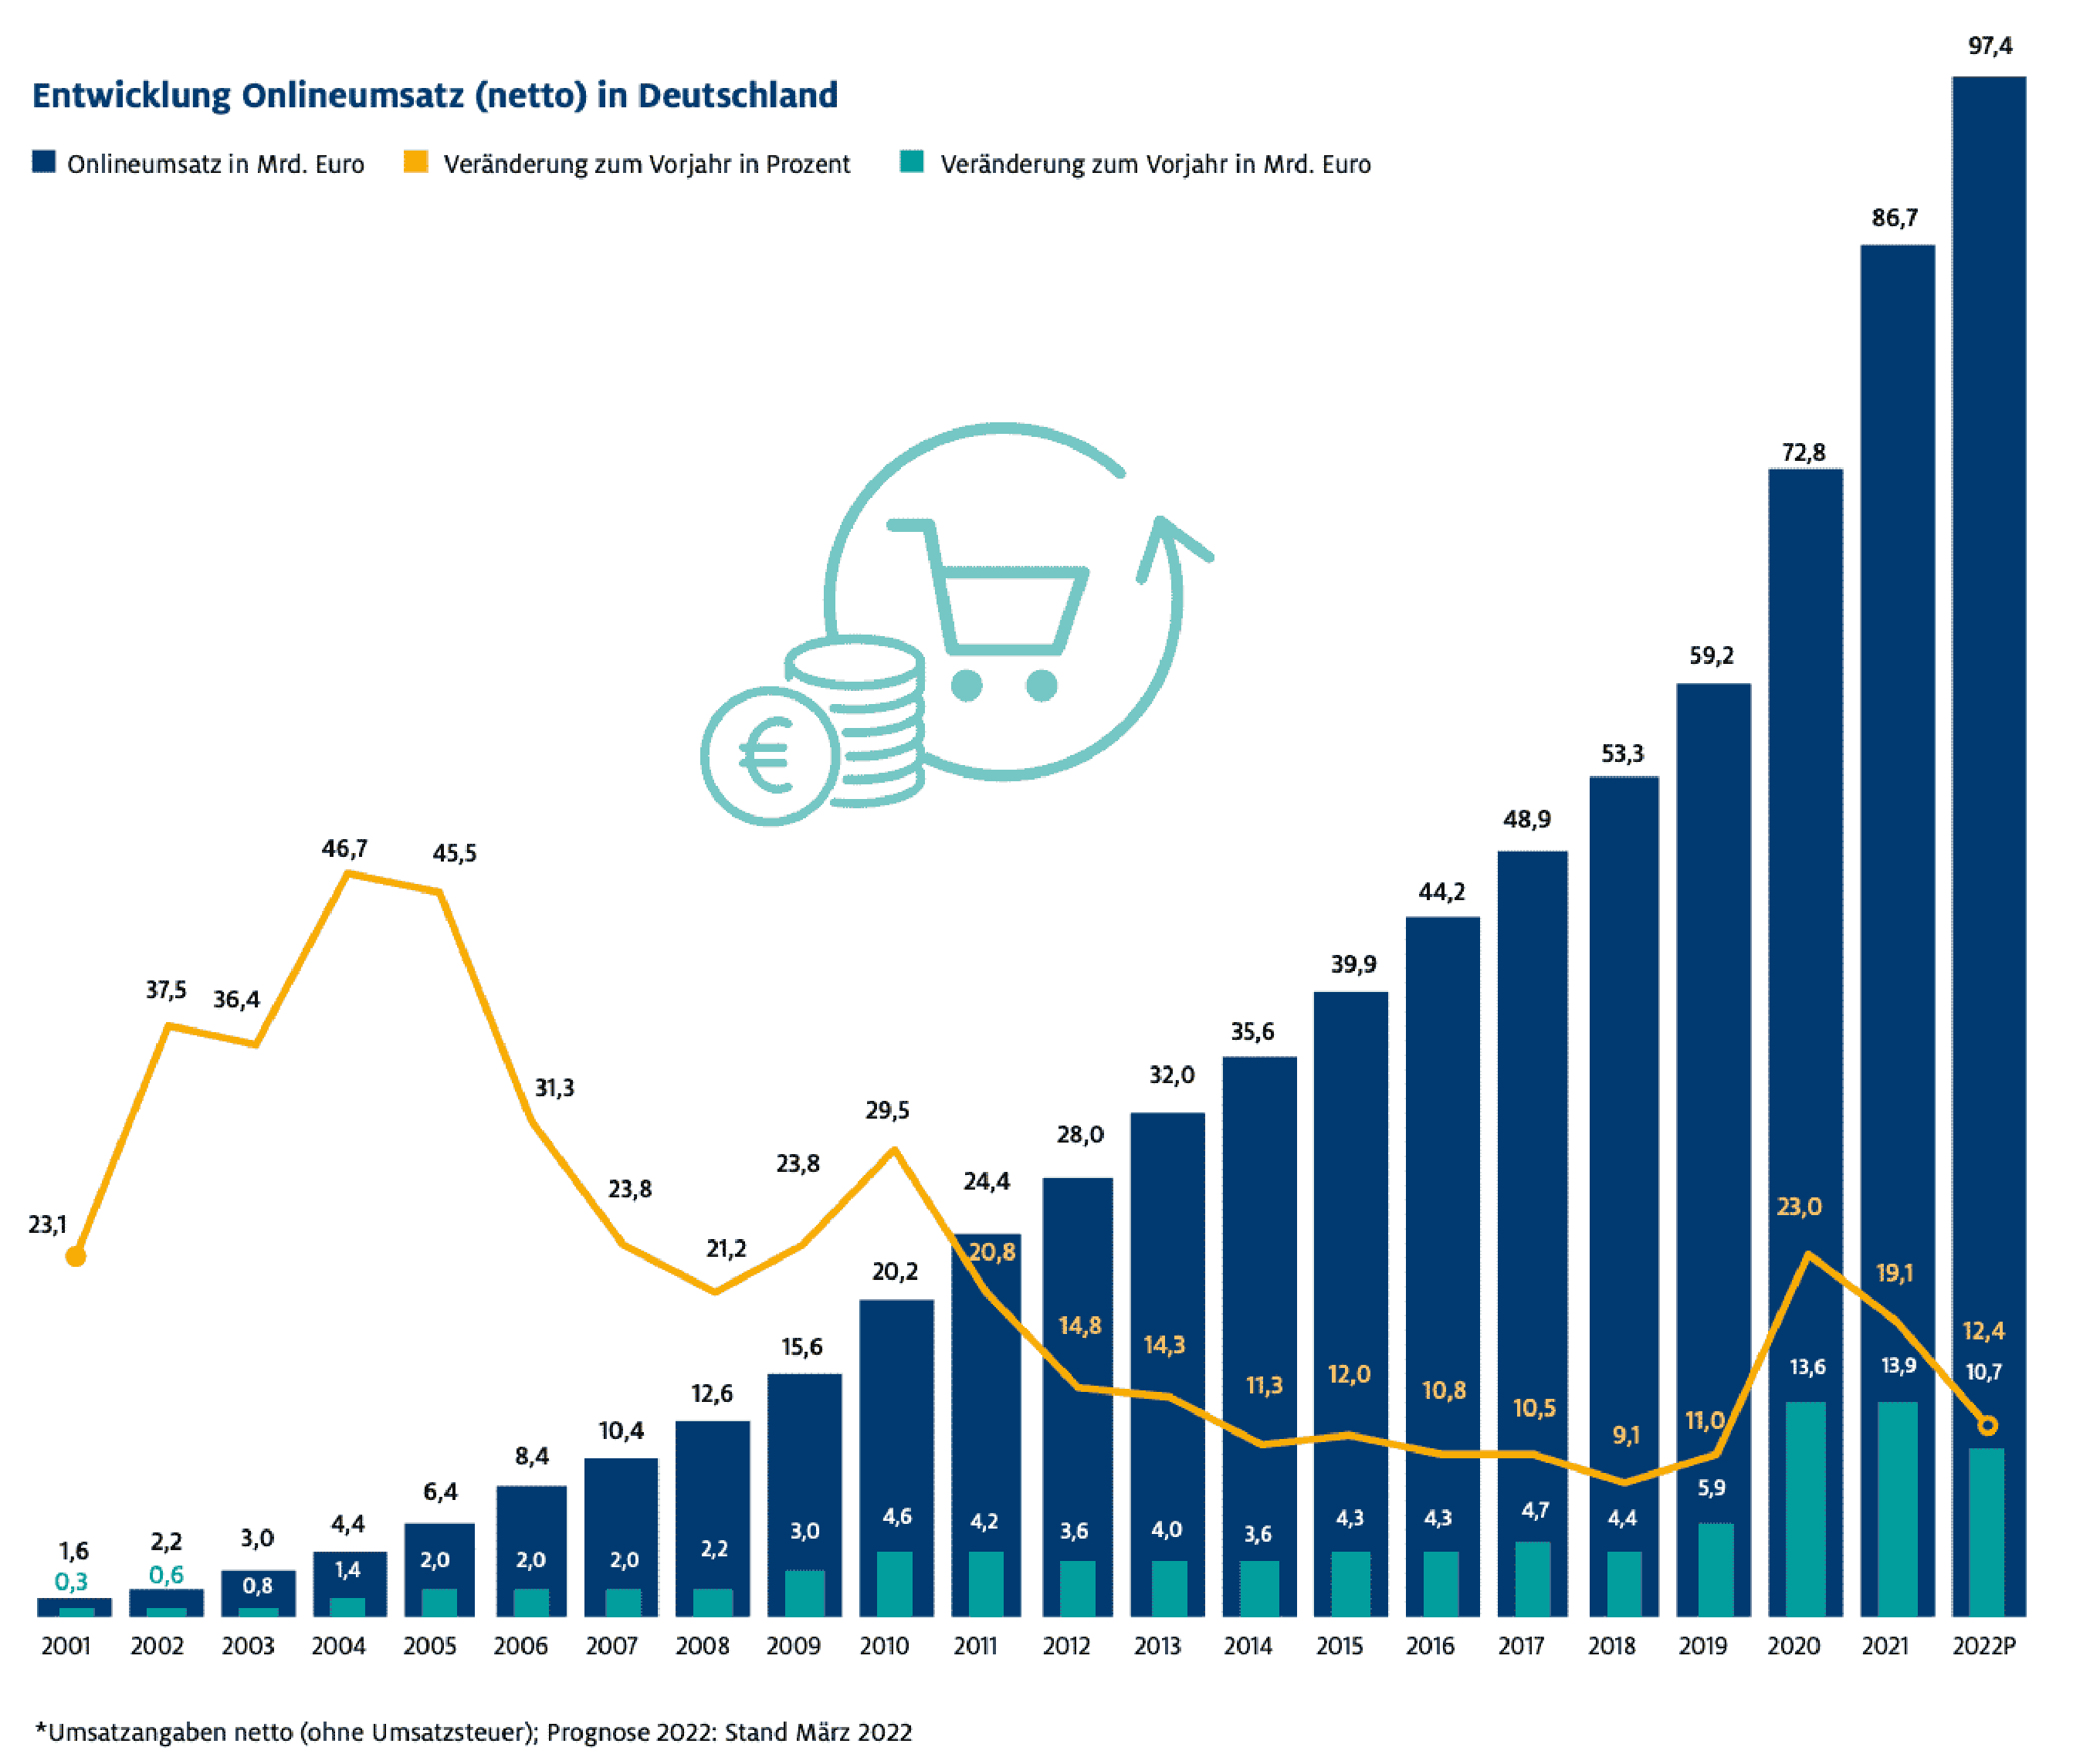
\includegraphics[width=\linewidth]{images/chapter1/umsatzprognose_2022.eps}
	\caption{Umsatzentwicklung E-Commerce von 2001-2022}
	\label{img:stat_prognose_2022}
\end{figure}

Mithilfe von Machine Learning können aus vorhandenen Daten, Nutzergruppe bestimmt werden, mit deren Hilfe besser Angebote für die Nutzergruppen erstellt und ausgespielt werden können.\vspace{0.2cm}

Allgemein benennt [\href{https://www.talend.com/de/resources/maschinelles-lernen}{talend.com}] folgende drei Vorteile für Unternehmen der durch den Einsatz von maschinellen Lernen entstehen.

\begin{enumerate}
	\item Future-Proof: es ist eine Technologie der Zukunft, die in den kommenden Jahren weiter entwickelt wird.
	\item Effizienz: durch die Automatisierung und Klassifizierung lassen sich große Datenmengen effizienter analysieren. Dadurch verbessern sich interne und externe Unternehmensprozesse.
	\item Fördert Konzentration: ML übernimmt repetitive Aufgaben, so bleibt Mitarbeitern für anspruchsvollere Arbeiten.
\end{enumerate}

\section{Motivation}
Im E-Commerce nutzen Onlineshop Betreiber Kundenklassifizierungen, um Kunden einzuteilen und ihnen besser Angebote unterbreiten zu können. Oft sind diese Klassifizierungen in den ersten Schritten bei der Shop-Planung oder bei einem \Gls{relaunch} erstellt wurden, basierend auf einer erwarteten und anvisierten Kundengruppe. In vielen Fällen werden keine Kundenklassifizierungen erstellt. Es wird unterstellt das alle Menschen zur Zielgruppe gehören.

\subsection{Ausgangslage}
Im Rahmen dieser Arbeit soll ein kleiner Onlineshop eines Verlages aus dem Nordosten Deutschlands untersucht werden. Über den Shop werden hauptsächlich Print-Produkte wie Bücher und Zeitschriften. Eine vorherige Planung und Analyse der Nutzergruppen und ihrer Bedürfnisse sind einigen Mitarbeitern, die den Shop betreuen, nicht wichtig.\vspace{0.2cm}

Folgende Aussagen trafen Mitarbeitern, die unmittelbar mit den Onlineshop Arbeiten und diesen betreuen.„Für den Onlineshop benötigen wir keine Nutzergruppen, dafür haben wir die verschiedene Menüpunkte. Nutzergruppen werden erst interessant, wenn wir auf verschiedenen Kanäle Werbung schalten.“ Aussage einer Mitarbeiterin für Kundenmanagement. „Zielgruppendefinition ist wichtig, aber für den Shop sollte keine angefertigt werden.“ Aussage einer Mitarbeiterin des Webdesigner Teams.

\subsection{Vorteile durch die Vorhersage}
Einer der wichtigsten Vorteile einer durch künstlicher Intelligenz vorhergesagten Nutzergruppenklassifizierung wäre das Ausschließen des menschlichen Einwirkens. Das Erhöht die Genauigkeit der Entscheidungen und es passieren weniger Fehler. Des Weiteren erkennt künstliche Intelligenz versteckte Muster aus tausenden und mehr Datensätzen. Ein weiterer Vorteil ist die Möglichkeit einer zeitnahen Anpassung der Verkaufsprozesse auf der Webseite und eine kontinuierliche Optimierung des Onlineauftritts.

\section{Ziel der Arbeit}
In dieser Arbeit ist die Prüfung, ob eine mögliche Vorhersage der Nutzergruppenklassifizierung durch künstliche Intelligenz möglich ist und ob diese Vorhersage Vorteile gegenüber einer klassischen Klassifizierung, beispielsweise durch Personas ist. Für die Vorhersage werden vorhandene Daten aus dem Shop und verschiedene externe Quellen verwendet.\vspace{0.2cm}

Durch die Zielsetzung lässt sich folgende Forschungsfrage und dazugehörige Unterfragen formulieren:\vspace{0.2cm}

„Ist die Erstellung eine Nutzergruppenklassifizierung mit Machine-Learning besser als eine klassische Analyse der Nutzergruppen?“

\begin{itemize}
	\item Welche Systeme und Algorithmen eignen sich am besten für die Klassifizierung?
	\item Sind die klassischen Nutzergruppen (z.B. mit soziodemografischen Merkmalen) aus E-Commerce noch relevant oder stehen andere Merkmale im Vordergrund?
\end{itemize}

\section{Inhaltlicher Aufbau der Arbeit}
Diesen Teil schreibe ich während der Fertigstellung der einzelnen Kapitel.
